\documentclass[sigconf, screen]{acmart}
% TODO: add algorithm or algorithm2e package for pseudo code 
\usepackage{custom}
\settopmatter{printacmref=false} % Removes citation information below abstract
\setcopyright{none} % Removes copyright statement
\renewcommand\footnotetextcopyrightpermission[1]{}
% \authorsaddresses{}


% \citestyle{acmauthoryear} %Citation support using author/year style
\begin{document}

\title{CRT: CUDA Ray Tracer}

\author{Raj Sugavanam}
\affiliation{
    \institution{Washington University in St. Louis}
    \city{}
    \state{}
    \country{}
}
\author{Junseo Shin}
\affiliation{
    \institution{Washington University in St. Louis}
    \city{}
    \state{}
    \country{}
}

% ABSTRACT
\begin{abstract}
    We present a spectral path tracer that showcases the capabilities and limits of the CUDA
    programming model in the field of physically based rendering. The simplest ray tracing
    algorithm requires the GPU to dispatch rays from the camera into the scene, and
    calculate the interaction of the rays with the scene geometry in order to render an output
    image of the camera's view. Our implementation focuses on rendering a Cornell box test scene
    to demonstrate the accuracy and performance of the CUDA ray tracer (CRT). Representing the
    scene geometry with triangle meshes presents the ability to interopt professional 3D modeling
    software with the ray tracer, but also explores the limitations of our implementation.
\end{abstract}

% FIRST FIGURE
\begin{teaserfigure}
    \centering
    \begin{subfigure}{0.24\textwidth}
        \centering
        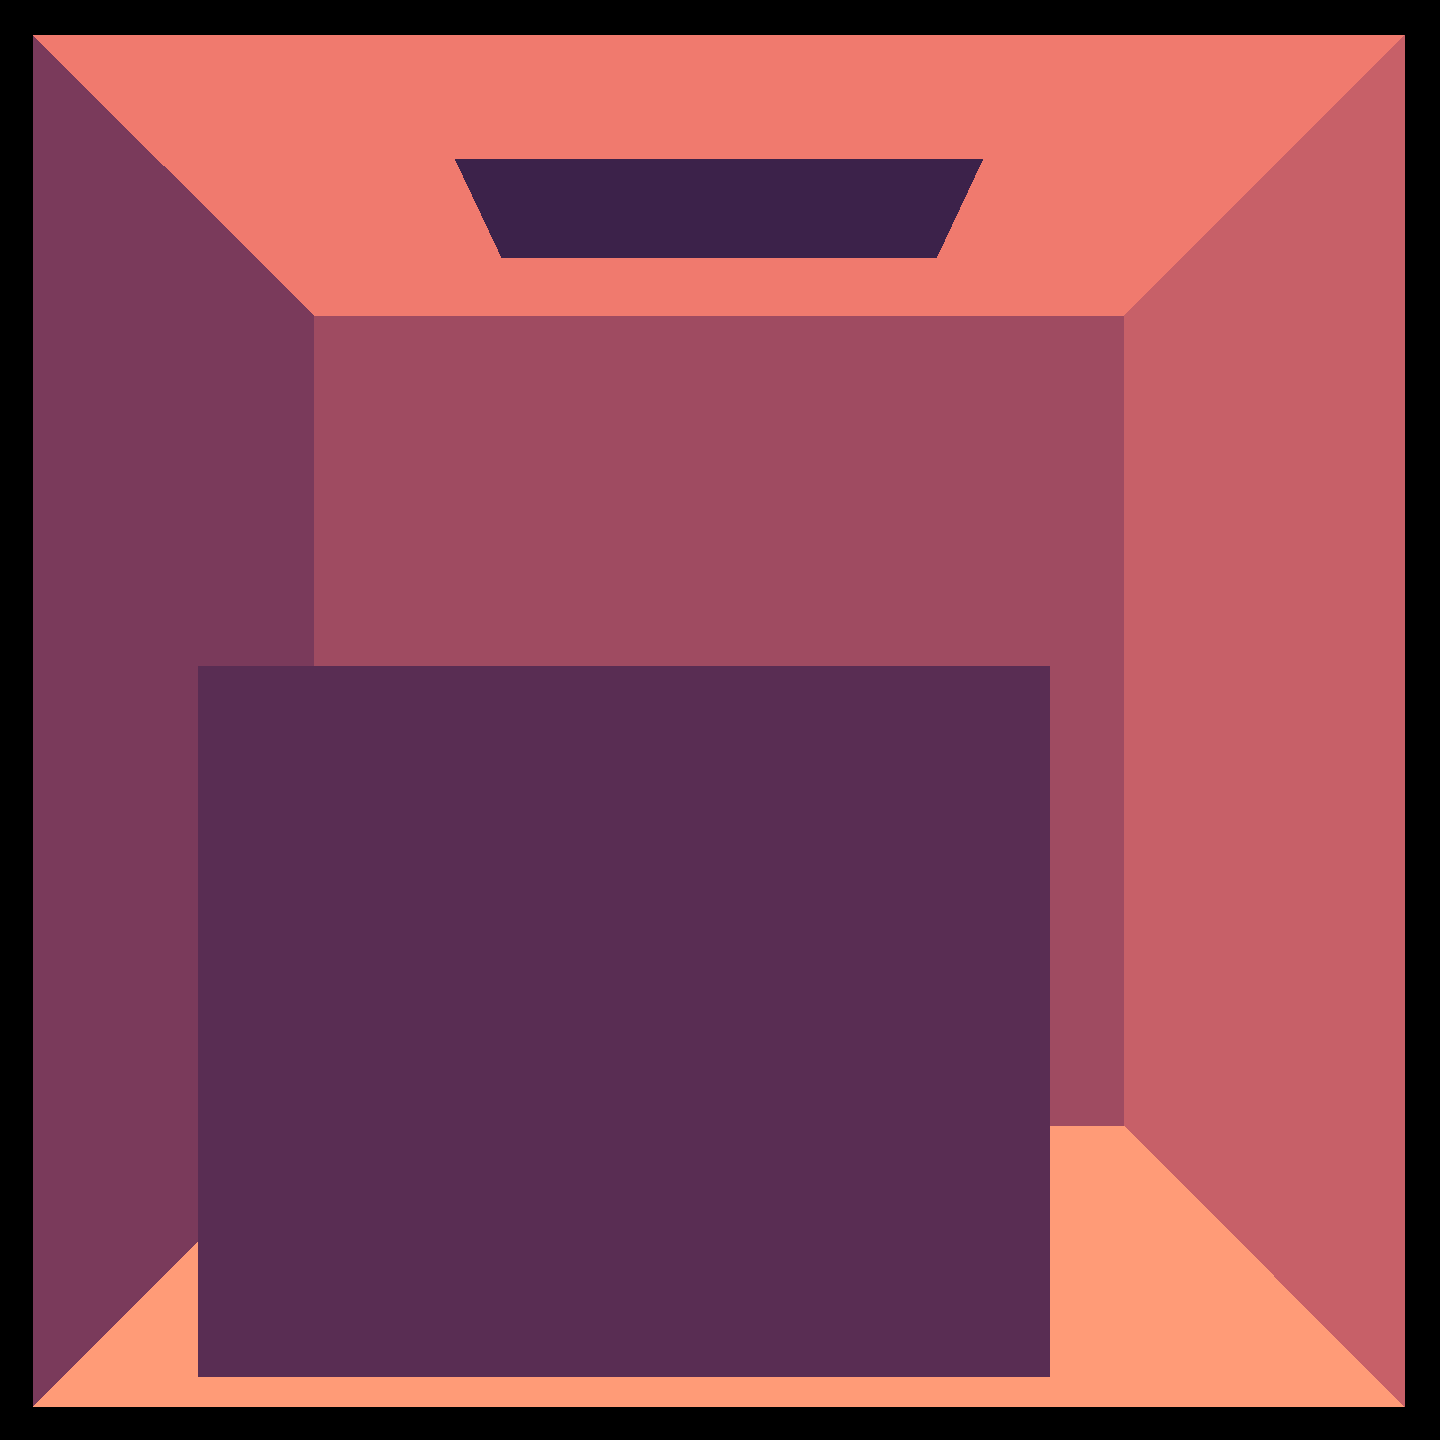
\includegraphics[width=\textwidth]{dk_box.png}
        % TODO: Change this
        \caption{something something}
        \Description{Image}
        \label{fig:teaser1}
    \end{subfigure}
    \begin{subfigure}{0.24\textwidth}
        \centering
        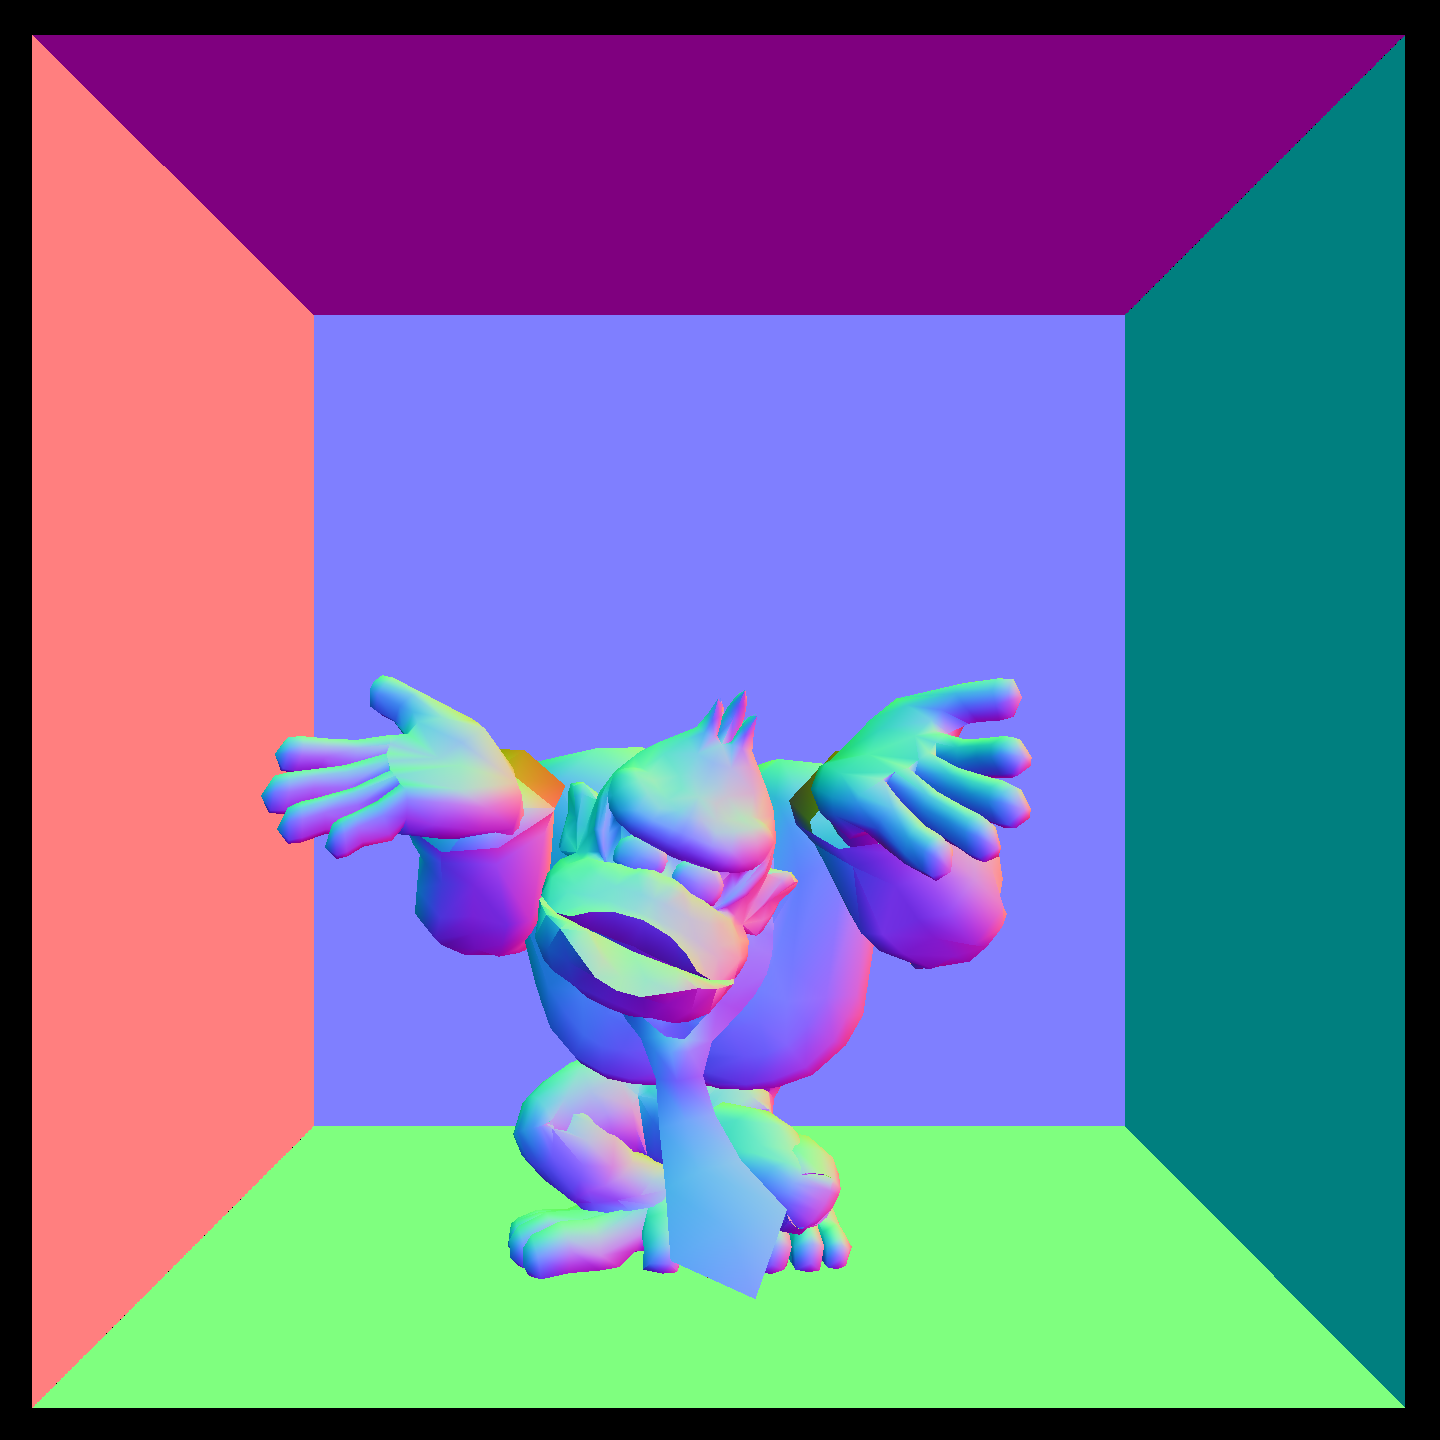
\includegraphics[width=\textwidth]{dk_normal_map.png}
        \caption{Normal map (smooth shading).}
        \Description{Image}
        \label{fig:teaser2}
    \end{subfigure}
    \begin{subfigure}{0.24\textwidth}
        \centering
        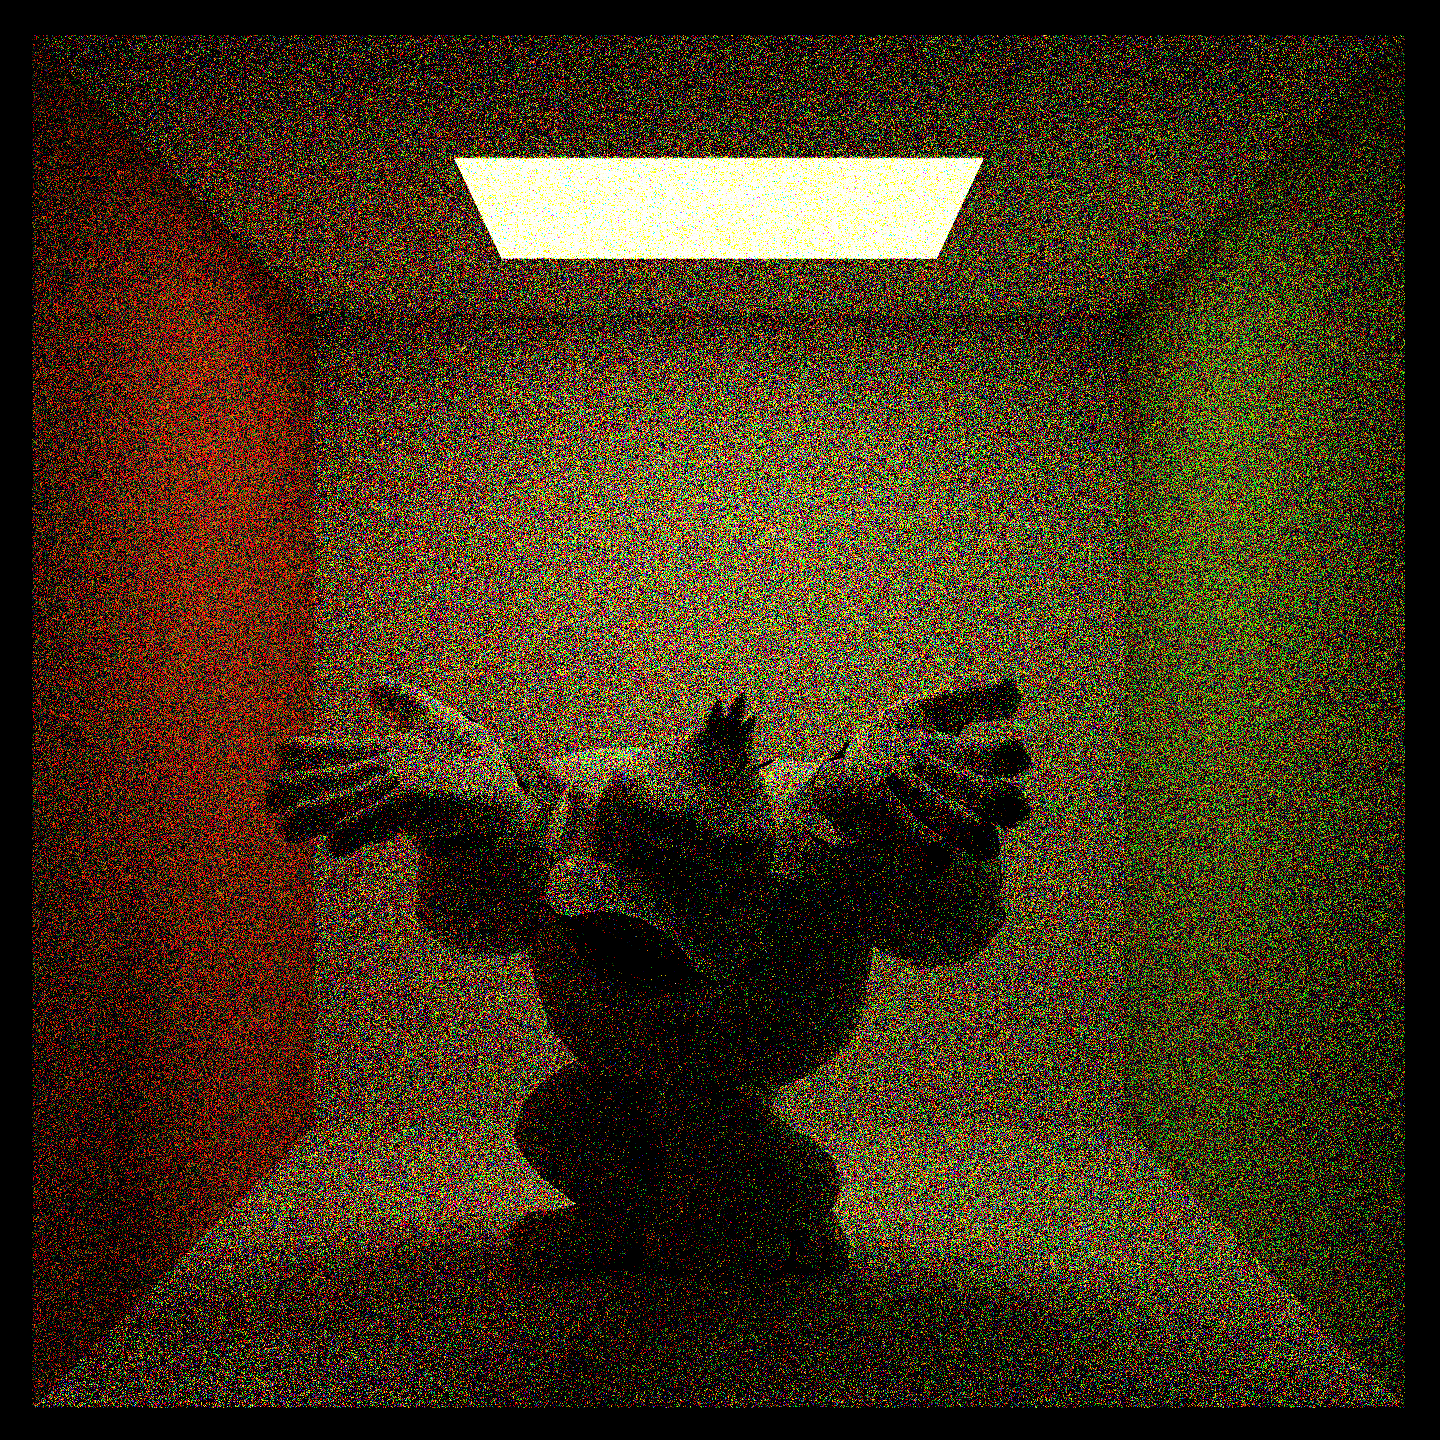
\includegraphics[width=\textwidth]{dk_16spp.png}
        \caption{Sparse samples, static light.}
        \Description{Image}
        \label{fig:teaser3}
    \end{subfigure}
    \begin{subfigure}{0.24\textwidth}
        \centering
        \includegraphics[width=\textwidth]{dk_256spp.png}
        \caption{Dense samples, static light.}
        \Description{Image}
        \label{fig:teaser4}
    \end{subfigure}
    \caption{something something}
    \Description{Image}
    \label{fig:teaser}
\end{teaserfigure}

\maketitle

% INTRO
\subfile{chapters/1_intro}
\subfile{chapters/2_problem_statement}
\subfile{chapters/3_approach}
\subfile{chapters/4_implementation}
\subfile{chapters/5_performance_measurements}
\subfile{chapters/6_optimizations_applied}
\subfile{chapters/7_results}
\subfile{chapters/8_discussion}
\subfile{chapters/9_conclusion}

% NEXT SECTION
% \newpage
\nocite{*}
\bibliographystyle{ACM-Reference-Format}
\bibliography{references}
\end{document}
